\section{Non-parametric regression}

\subsection{Explaining the code:}
 The code contains a NadarayaWatsonRegressor class and three kernel types that can be used - Gaussian, Epachnikov and Square (Tophat). Let us suppose our model is called \lq\lq regressor\rq\rq. We first need regressor to store our data, which is done by calling regressor.fit(X, Y). regressor.display(bandwidth) plots the estimated KDE for the particular bandwidth.\\
 Noticing that the data we have been given has a range of x values which are greater than 0 and less than 4, I have taken these as my limits for plotting.\\
 Within the range of min(X) to max(X), we plot values corresponding to the y\_labels given (note again that I am using the fact that the x values in the graph are already very dense, in order to save on computation). Outside this range, I plot the estimated y\value every 0.001 units.\\
 regressor.plot\_cross\_validator(bandwidths) can be used to generate a plot of cross-validation scores. Assumptions made here include the assumption that bandwidths is an array of non-zero values and is in increasing order. While trying to find the optimal bandwidth, plot\_cross\_validator() was called with bandwidths being np.linspace(0.1, 2, 200)\\
 Finally, regressor.display\_4\_plots can be used to generate the picture required by the assignment. The user needs to pass as arguments the bandwidths he wants to assign to the top left, top right and bottom left graphs respectively. For instance, I have called regressor3.display\_4\_plots(0.01, 1.75, 0.32) to represent that h=0.01 leads to overfitting and undersmoothening, h=1.75 leads to underfitting and oversmoothening and h=0.32 seems optimal based on cross validation scores.

\subsection{Bandwidth corresponding to minimum estimated risk: }
For a Gaussian kernel, the computed optimal bandwidth was 0.13.\\
For a Epachnikov kernel, the computed optimal bandwidth was 0.32.\\
For a Tophat/Square kernel, the computed optimal bandwidth was 0.31.
\begin{figure}[H]
    \centering
    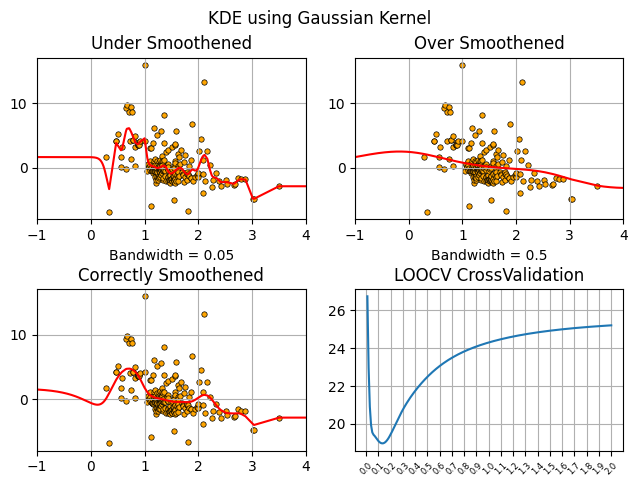
\includegraphics[width=0.5\textwidth]{../q4/gaussian_kernel_regression.png}
    \caption{Gaussian Kernel Regression - undersmoothening, oversmoothening, optimal bandwidth and Cross Validation curve}
    \label{fig:q4_1}
\end{figure}
\begin{figure}[H]
    \centering
    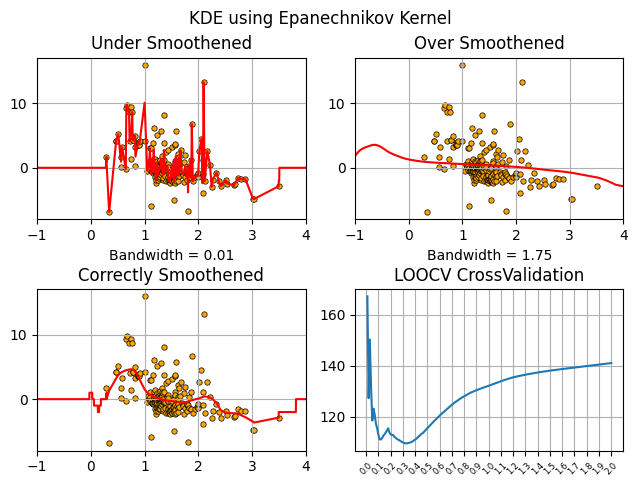
\includegraphics[width=0.5\textwidth]{../q4/epanechnikov_kernel_regression.png}
    \caption{Epachnikov Kernel Regression - undersmoothening, oversmoothening, optimal bandwidth and Cross Validation curve}
    \label{fig:q4_2}
\end{figure}
\begin{figure}[H]
    \centering
    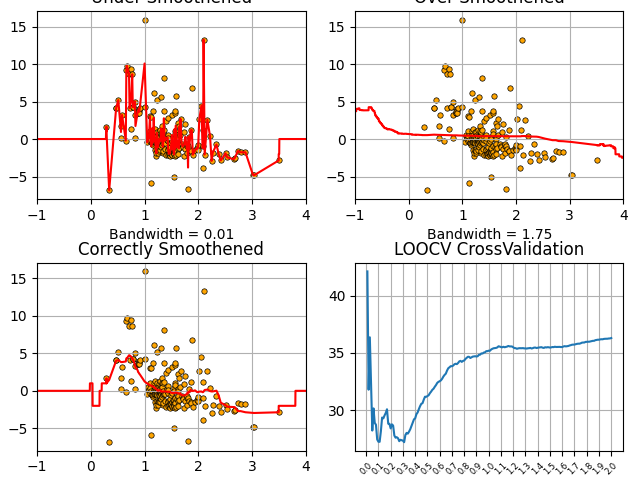
\includegraphics[width=0.5\textwidth]{../q4/tophat_kernel_regression.png}
    \caption{Tophat Kernel Regression - undersmoothening, oversmoothening, optimal bandwidth and Cross Validation curve}
    \label{fig:q4_3}
\end{figure}
\subsection{Comments on similarity and dissimilarity}
 The Gaussian estimator seems a lot smoother than the others, especially compared to Tophat, presumably because of the gaussian kernel itself being smooth and not jerky like the tophat kernel.\\
 The Gaussian estimator has a lower optimal bandwidth, presumably because it assigns a non-zero weight to all points, thus even points which are far away have some smoothening influence, whereas with Epachnikov or Tophat, both of which have finite support, we need a larger bandwidth in order to capture enough neighboring points for a smooth estimate.\\
 The EPA and Tophat estimators do not have as smooth cross-validation curves as the Gaussian, presumably because they are abrupt jumps in the risk when a transition between bandwidths causes one object to lose all influence over the kernel at a point.
\newpage